\lecture[Diskrete Zufallsvariablen. Massefunktion. Bernoulli - Binomialverteilung. Unabhängigkeit von Ereignissen. Poissonverteilung.]{Mi 21 Apr 2021 10:15}{Zufallsvariablen, Wahrscheinlichkeitsverteilungen}
\subsection{Zufallsvariablen}
Wir werden Funktionen der Ergebnisse betrachten:
\begin{definition}[Diskeret Zufallsvariable]\label{def:diskrete-zufallsvariable}
    Sei $(\Omega, \mathcal{F}, \mathbb{P})$ ein Wahrscheinlichkeitsraum. Eine \vocab{diskrete Zufallsvariable} ist eine \underline{messbare} Abbildung
    \[
    X : \Omega \longrightarrow \mathcal{S}
    .\] 
    mit $\mathcal{S}$ abzählbar (denke: 'diskret'). \\
    Messbar bedeutet hierbei, dass
    \[
        \forall s\in \mathcal{S} \colon X^{-1}(s) = \left \{\omega\in \Omega\mid  X(\omega) = s\right\} \in  \mathcal{F}
    .\] 
\end{definition}
\begin{notation}
    Wir schreiben auch kurz:
    \[
        X^{-1}(s) = \left \{X(\omega) = s\right\}  = \left \{X = s\right\} 
    .\] 
\end{notation}

\begin{figure}[ht]
    \centering
    \incfig{diskrete-zufallsvariable}
    \caption{Diskrete Zufallsvariable}
    \label{fig:diskrete-zufallsvariable}
\end{figure}
\begin{definition}
    Sei $(\Omega, \mathcal{F}, \mathbb{P})$ ein Wahrscheinlichkeitsraum  und $X : \Omega\to \mathcal{S}$ eine diskrete Zufallsvariable. \\
    Die \vocab{Verteilung von $X$} ist die Wahrscheinlichkeitverteilung $\mu_X$ auf  $\mathcal{S}, \mathcal{P}(\mathcal{S}) = \tilde{F}$, s.d. $\forall B\in \tilde{F}: \mu_X(B) := \mathbb{P}(X^{-1}(B))$. \\
    $\mu_X$ hat eine \vocab{Massenfunktion}
     \[
         p_{X}(s) := \mathbb{P}
    .\] 
\end{definition}
\begin{example}[Werfen von $n$ Münzen]
    Betrachte folgende Situation:
    \begin{itemize}
        \item Sei $\Omega = \left \{\omega = (\omega_1,\ldots,\omega_n \mid \omega_i \in \left \{0,1\right\} \text{ für } 1\leq i\leq n\right\}$, wobei
\[
\omega_k = \begin{cases}
    0 & \text{falls $k$-ter Wurf ist Zahl} \\
    1 & \text{falls $k$-ter Wurf ist kopf}
\end{cases}
.\] 

\item Und sei $\mathcal{F} = \mathcal{P}(\Omega)$ und $\mathbb{P}$ die Gleichverteilung.
    \end{itemize}
    \begin{enumerate}[(1)]
        \item Setze
                \begin{equation*}
                X_k: \left| \begin{array}{c c l} 
                \Omega & \longrightarrow & \mathcal{S} = \left \{0,1\right\}  \\
                \omega & \longmapsto &  \omega_k
                \end{array} \right.
            \end{equation*}
            für $k = 1,\ldots,n$. Dies ist eine diskrete Zufallsvariable mit Verteilung $\mu_{X_k}$ mit
            \[
                p_{X_k}(s) = \mathbb{P}(X_k = s) = \frac{2^{n-1}}{2^n} = \frac{1}{2}
            .\] 
            Wir sehen also, dass $X_k$ gleichverteilt ist.
        \item Definiere
                \begin{equation*}
                Y: \left| \begin{array}{c c l} 
                \Omega & \longrightarrow & \mathcal{S} := \left \{0,1,\ldots,n\right\}  \\
                \omega & \longmapsto &  \omega_1 + \ldots + \omega_n
                \end{array} \right.
            \end{equation*}
            d.h.
            \[
                Y(\omega) = \# \left \{\text{geworfene Köpfe}\right\} 
            .\] 
    Es hat nun $\mu_Y$ die Massenfunktion:
    \[
        p_Y(k) = \frac{1}{2^n} \abs{\left \{\omega \mid  w_1 + \ldots + \omega_n = k\right\} } = \frac{\binom{n}{k}}{2^n}
    .\] 
    Diese Verteilung sieht wie folgt aus: \\
    \begin{minipage}{\textwidth}
        \centering
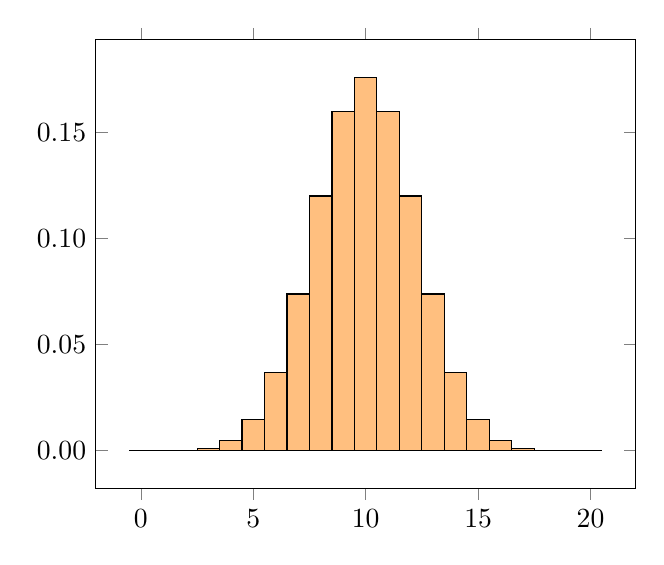
\begin{tikzpicture}[
    declare function={binom(\k,\n,\p)=\n!/(\k!*(\n-\k)!)*\p^\k*(1-\p)^(\n-\k);}
]
\begin{axis}[
    samples at={0,...,20},
    yticklabel style={
        /pgf/number format/fixed,
        /pgf/number format/fixed zerofill,
        /pgf/number format/precision=2
    },
    ybar=0pt, bar width=1
]
\addplot [fill=orange, fill opacity=0.5] {binom(x,20,0.5)};
\end{axis}
\end{tikzpicture}
\captionof{figure}{Massenfunktion $p_Y(k)$}
    \end{minipage} \\
    Diese sind Sonderfälle der Bernoulliverteilung und der Binomialverteilung.
    \end{enumerate}
\end{example}

\subsubsection{Die Bernoulli-Verteilung}
\begin{definition}[Bernoulli-Verteilung]\label{def:bernoulli-verteilung}
    Sei $p\in [0,1]$ gegeben. Die Wahrscheinlichkeitsverteilung auf $\left \{0,1\right\} $ mit Massenfunktion
    \[
        p(k) = \begin{cases}
            p & k = 1 \\
            1-p & k = 0
        \end{cases}
    .\] 
        heißt \vocab{Bernoulli-Verteilung mit Parameter $p$}. 
\end{definition}
\begin{notation}
    Wir notieren $\operatorname{Ber} (p)$ für die Bernoulli-Verteilung mit Parameter $p$.
\end{notation}
\begin{example}
    \begin{enumerate}[label=\protect\circled{\alph*}]
        \item Sei eine Münze gegeben, die mit Wahrscheinlichkeit $p$ Kopf zeigt. Hier ist
             \[
                 \Omega = \left \{\text{Zahl}, \text{Kopf}\right\} \qquad \mathbb{P}(\text{Kopf}) = p = 1-\mathbb{P}(\text{Zahl})
            .\] 
            Sei
            \[
                X(\omega) = \begin{cases}
                    1 & \omega = \text{Kopf} \\
                    0 & \omega = \text{Zahl}
                \end{cases}
            .\] 
            Dann ist $\mathbb{P}(X = 1) = p$ und $X \sim  \operatorname{Ber} (p)$.
            \begin{notation}
                Wir schreiben $X \sim \Ber(p)$, wenn $X$ die Verteilung  $\Ber(p)$ hat.
            \end{notation}
        \item In einer Urne befinden sich $n$ blaue Kugeln und  $m$ rote Kugeln. Wir ziehen eine Kugel aus der Urne (Annahme: Gleichverteilung). Dann ist
            \[
                \Omega = \left \{\omega = (\omega_1,\ldots,\omega_{n+m}) \mid \omega_i \in  \left \{\text{blau},\text{rot}\right\} \text{ mit $n$ mal blau} \right\} 
            .\] 
            Setze $\mathcal{F}= \mathcal{P}(\Omega)$ und wähle $\mathbb{P}$ als die Gleichverteilung. Betrachte
            \[
                X(\omega) = \begin{cases}
                    1 & \text{falls $\omega_i$ ist blau} \\
                    0 & \text{sonst}
                \end{cases}
            .\] 
Diese hat also die Verteilung
\[
    \mathbb{P}(X = 1) = \frac{\binom{m+n-1}{n-1}}{\binom{m+n}{n}} = \frac{(m+n-1)!}{(n-1)! m!} \frac{n! m!}{(m+n)!} = \frac{n}{m+n}
.\] 
Also ist $X \sim \Ber\left( \frac{n}{n+m} \right) $.
    \end{enumerate}
\end{example}

\subsubsection{Die Binomial-Verteilung}
\begin{definition}[Binomial-Verteilung]\label{def:binomial-verteilung}
    Seien $n\in \N$ und $p\in [0,1]$ gegeben. Die Wahrscheinlichkeitsverteilung auf $\left \{0,1,\ldots,n\right\} $ mit Massenfunktion
    \[
        p(k) = \binom{n}{k}p^k(1-p)^{n-k}
    .\] 
    für $k=0,\ldots,n$ heißt \vocab{Binomialverteilung mit Parametern $n$ und  $p$}. 
\end{definition}
\begin{notation}
    Wir notieren $\Bin(n,p)$ für die Binomialverteilung mit Parametern  $n$ und  $p$.
\end{notation}

\begin{example}[Ziehen mit Zurücklegen]
    \begin{itemize}
        \item Seien $m$ Kugeln in einer Urne, davon  $p\cdot m\in \N$ weiße Kugeln und $(1-p)m$ schwarze Kugeln.
        \item Wir ziehen eine Kugel, notieren uns die Farbe und legen sie wieder zurück.
        \item Wir mischen die übrigen Kugeln wider gut.
        \item Wir wiederholen die vorherigen Schritte, bis wir $n$ Ziehungen durchgeführt haben.
        \item Dies modellieren wir durch
            \[
            \Omega = \left \{0,1\right\} ^n
            .\] 
            wobei $\omega=(\omega_1,\ldots,\omega_n) \in \Omega$ gegeben ist durch
            \[
            \omega_i = \begin{cases}
                1 & \text{falls Farbe der $i$-ten Kugeln weiß ist} \\
                0 &\text{sonst}
            \end{cases}
            .\] 
        \item Sei nun $X(\omega) = \sum_{k=1}^n \omega_k = \# \left \{\text{weiße Kugeln} \right\} $.
    \end{itemize}
    Dann behaputen wir, dass $X \sim  \Bin(n,p)$. In der Tat gilt:
    \begin{equation}
        \begin{split}
            \frac{\abs{\omega\in \Omega \mid  X(\omega) = l}}{\abs{\Omega} } &= \frac{\binom{n}{l} \cdot  (pm)^{l}\left( (1-p)m \right)  ^{n-l}}{m^n} \\
                                                                             &= \frac{\binom{n}{l}p^l (1-p)^{n-l}\cdot m^n}{m^n} = \binom{n}{l}p^l(1-p)^{n-l}
        \end{split}
    \end{equation}
\end{example}
\begin{remark}
Wir haben hier den Begriff der \vocab{Unabhängigkeit} genutzt, den wir nun genauer kennenlernen wollen.
\end{remark}
\begin{definition}[Unabhängige Ereignisse]\label{def:unabhängige-ereignisse}
    Sei $(\Omega, \mathcal{F}, \mathbb{P})$ ein Wahrscheinlichkeitsraum. Die Ereignisse $E_1,E_2,\ldots,E_n$ heißen \vocab{unabhängig}, falls
    \[
        \mathbb{P}(E_{i_1} \cap E_{i_2} \cap \ldots \cap E_{i_k}) = \prod_{l=1}^k \mathbb{P}(E_{i_l})
    .\] 
    für alle $2\leq k\leq n$ und $1\leq i_1<i_2 < \ldots < i_k \leq n$.
\end{definition}

\begin{example}
    \begin{itemize}
        \item 
    Betrachte zwei Würfelwürfe, d.h. $\Omega = \left \{1,\ldots,6\right\} ^2$ und notiere $\omega = (\omega_1,\omega_2)$. Dann können wir
    \[
    E_1 = \left \{\omega_1 = 3\right\}  \qquad E_2 = \left \{\omega_2 \geq  4\right\} 
    .\] 
    betrachten. Wir rechnen nach, dass
    \[
        \mathbb{P}(\omega_1 = 3 \cap \omega_2 \geq  4 ) = \frac{3}{36} = \frac{1}{6}\cdot \frac{3}{6} = \mathbb{P}(\omega_1 = 3) \cdot \mathbb{P}(\omega_2 \geq  4)
    .\] 
    also sind die beiden Ereignisse unabhängig voneinander. Das macht auch semantisch Sinn, weil wir durch das Ergebnis des ersten Würfelwurfs keine Informationen über das Ergebnis des zweiten Würfelwurfs erhalten.
\item

Falls $E_1,E_2,\ldots,E_n$ unabhängige Ereignisse sind mit $\mathbb{P}(E_i) = p$ für $1\leq i\leq n$, dann gilt
\[
    \mathbb{P}(\text{genau $k$ der Ereignisse treten ein}) = \binom{n}{k} p^k (1-p)^{n-k}
.\] 
Dies rechnen wir nach. Setze hierzu 
\[
    A_{(i_1,\ldots,i_k)} = \left \{\omega\in \Omega \mid  E_{i_1},\ldots,E_{i_k} \text{ treten ein, die anderen nicht}\right\}
\]
Dann ist
\[
\tilde{A} = \bigsqcup_{1\leq i_1<\ldots<i_k \leq n} A_{i_1,\ldots,i_k}
.\] 
eine disjunkte Vereinigung, also erhalten wir
\begin{equation}
    \begin{split}
        \mathbb{P}(\tilde{A})                                 &= \sum_{1\leq i_1<\ldots<i_k\leq n} \mathbb{P}(A_{(i_1,\ldots,i_k}) \\
                                                              &\stackrel{\text{unabhängig}}{=} \sum_{1\leq i_1<\ldots<i_k \leq n} \prod_{j\in \left \{i_1,\ldots,i_k\right\} } \mathbb{P}(E_j) \cdot \prod_{l \not\in \left \{i_1,\ldots,i_k\right\} } \mathbb{P}(E_l^{c}) \\
                                                              &= \sum_{1\leq i_1<\ldots<i_k \leq n} p^k(1-p)^{n-k} \\
                                                              &= \binom{n}{k} p^k (1-p)^{n-k}
    \end{split}
\end{equation}
    \end{itemize}
\end{example}
\begin{remark}
    Streng genommen haben wir in der letzten Rechnung verwendet, dass mit $E_1,\ldots,E_n$ unabhängig auch $F_1,\ldots,F_n$ für $F_i = E_i $ oder  $F_i = E_i ^{c}$ unabhängig voneinander sind. Dies müssten wir noch einmal nachrechnen. Für den Fall $n=2$ ist z.B:
     \[
         \mathbb{P}(E_1 \cap E_2^{c}) + \mathbb{P}(E_1 \cap E_2) = \mathbb{P}(E_1 \cap (E_2 \cup E_2^{c}) = \mathbb{P}(E_1)
    .\] 
    Also ergibt sich
    \[
        \mathbb{P}(E_1\cap E_2^{c}) = \mathbb{P}(E_1) - \mathbb{P}(E_1)\mathbb{P}(E_2) = \mathbb{P}(E_1)(1-\mathbb{P}(E_2) = \mathbb{P}(E_1) \mathbb{P}(E_2^{c})
    .\] 
    wie zu zeigen war.
\end{remark}
\subsubsection{Die Poisson-Verteilung}
Betrachte Ereignisse $E_1,\ldots,E_n$, die unabhängig voneinander sind und jeweils Wahrscheinlichkeit $p$ haben. Wir skizzieren dies mit \tikz \fill[blue] circle (2pt); für ein eingetretenes Ereignis und \tikz \fill[red] circle (2pt); für das Nicht-Eintreten des entsprechenden Ereignisses \\
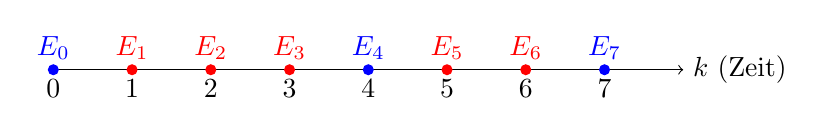
\begin{tikzpicture}
    \draw[->] (0,0) -- (8,0) node[anchor=west] {$k$ (Zeit)};
    \foreach \x in {1,2,3,5,6} {
        \fill[red] (\x,0) node[anchor = north,black]{$\x$} node[anchor=south] {$E_{\x}$} circle (2pt);
    }
    \foreach \x in {0,4,7} {
        \fill[blue] (\x,0) node[anchor = north,black]{$\x$} node[anchor=south] {$E_{\x}$} circle (2pt);
    }
\end{tikzpicture}
\begin{question}
    Was passiert, wenn $n\gg 1$, d.h. wie viele Erfolge werden wir (ca.) unter diesen $n$ Ereignissen haben?
\end{question}
Typischerweise haben wir dann $\mathcal{O}(pn)$ Erfolge in $E_1,\ldots,E_n$. Die Erfolgswahrscheinlichkeit $p$ hänge nun von  $n$ ab, d.h.  $p = p(n)$. Wir wollen den Erwartungswert  $p\cdot n$ festhalten und $n$ groß werden lassen, d.h. sei  $λ\in (0,\infty)$ so, dass 
\[
    \lim_{n \to \infty} p(n)\cdot n = λ
.\] 
Wir können uns das Ganze so vorstellen, dass wir in einem Zeitintervall von $1$ erwarten, dass $λ$ Ereignisse eintreten und wir nun mit einem kleinen Zeitintervall $\delta = \frac{1}{n}$ für große $n$ das kontinuierliche Zeitintervall durch  $n$ unabhängige Ereignisse ersetzen, die jeweils mit Wahrscheinlichkeit  $\frac{λ}{n}$ eintreten und uns nun fragen, wie wahrscheinlich es also ist, dass wir eine gewisse Anzahl an Ereignissen im Zeitintervall beobachten. \\
\noindent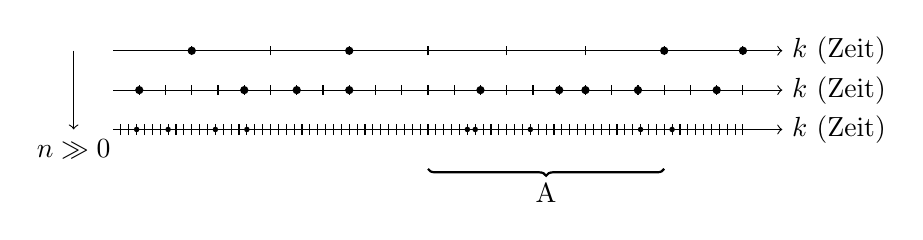
\begin{tikzpicture}
    \draw[->] (0,1) --(8.5,1) node[anchor=west] {$k$ (Zeit)};
    \foreach \x in {1,...,8} {
        \draw (\x,0.94) -- (\x,1.06);
    }
    \foreach \y in {1,3,7,8} {
        \fill (\y,1) circle (1.5pt);
    }
    \draw[->] (0,0.5) --(8.5,0.5) node[anchor=west] {$k$ (Zeit)};
    \foreach \x in {1,...,24} {
        \draw (\x/3,0.44) -- (\x/3,0.56);
    }
    \foreach \y in {1,5,7,9,14,17,18,20,23} {
        \fill (\y/3,0.5) circle (1.5pt);
    }
    \draw[->] (0,0) --(8.5,0) node[anchor=west] {$k$ (Zeit)};
    \foreach \x in {1,...,80} {
        \draw (\x/10,-2pt) -- (\x/10,2pt);
    }
    \foreach \y in {3,7,13,17,45,46,53,67,71} {
        \fill (\y/10,0) circle (1pt);
    }
\draw [
    thick,
    decoration={
        brace,
        mirror,
        raise=0.5cm
    },
    decorate
    ] (4,0) -- (7,0) node[midway,yshift=-23pt]{A};
\draw[->] (-0.5,1) -- (-0.5, 0) node[anchor=north] {$n \gg 0$};
\end{tikzpicture} \\
Es stellt sich also
\begin{question}
    Was ist für ein Zeitintervall $A$ die Wahrscheinlichkeit, dass wir im Intervall genau  $k$ Ereignisse beobachten, d.h. was ist
     \[
         \lim_{n\to \infty} \mathbb{P}(\exists k \text{ Erfolge in }  A)
    .\] 
    ?
\end{question}
\begin{itemize}
    \item Sei $p=p(n)$ sodass  $\lim_{n \to \infty} pn = λ \in (0,\infty)$.
    \item Wähle Zeiteinheit $\delta = \frac{1}{n}$.
\end{itemize}
Die Antwort gibt der folgende Satz.
\begin{theorem}\label{thm:poisson-verteilung-als-limes-von-binomialverteilungen}
    Sei $λ\in (0,\infty)$. Dann ist
    \[
        \lim_{n \to \infty} \Bin\left(n, \frac{λ}{n}\right) (k) = \frac{e^{-λ}λ^k}{k!}
    .\] 
    für $k=0,1,2,\ldots$
\end{theorem}
\begin{proof}
    Sei $k$ fest. Dann ist
    \begin{equation}
        \begin{split}
            \Bin\left(n, \frac{λ}{n}\right)(k) &= \frac{n!}{(n-k)^ k!} \left(\frac{λ}{n}\right)^k \left( 1-\frac{λ}{n} \right)^{n-k} \\
                                               &= \underbrace{\frac{n(n-1)\cdot \ldots(n-k+1)}{n^k}}_{\to 1} \frac{λ^k}{k!} \underbrace{\left( 1-\frac{λ}{n} \right) ^{n}}_{\to e^{-λ}} \underbrace{\left( 1-\frac{λ}{n} \right) ^{-k}}_{\to (1-0)^{-k} =1} \\
                                               &= \frac{λ^k}{k!} \cdot e^{-λ}
        \end{split}
    \end{equation}
\end{proof}
\begin{definition}[Poisson-Verteilung]\label{def:poisson-verteilung}
    Sei $λ\in (0,\infty)$ fest. Die Wahrscheinlichkeitsverteilung auf $\left \{0,1,2,\ldots\right\} $ mit Massenfunktion
    \[
        p(k) = \frac{e^{-λ λ^k}}{k!}
    .\] 
    heißt \vocab{Poisson-Verteilung mit Parameteter $λ$}. 
\end{definition}
\begin{notation}
    Wir schreiben auch $\Poi(λ)$ für die Poisson-Verteilung zum Parameter $λ$.
\end{notation}









